\documentclass[11pt,a4paper]{scrartcl}
\usepackage[T1]{fontenc}
\usepackage{microtype}
\usepackage{lmodern}
\usepackage{amsmath}
\usepackage{amsfonts}
\usepackage{amssymb}
\usepackage{enumerate}
\usepackage{graphicx}
\usepackage{float}

\usepackage{listings}
\usepackage{color}
%% http://stackoverflow.com/questions/741985/latex-source-code-listing-like-in-professional-books
\usepackage{courier}
\definecolor{light-gray}{gray}{0.95}
\lstset{
  % language=C,
  basicstyle=\small\sffamily,
%   basicstyle=\small\ttfamily,
  numbers=left,
  numberstyle=\tiny,
  frame=tb,
%  columns=fullflexible,
%  showstringspaces=false,
	backgroundcolor=\color{light-gray},
	linewidth=\linewidth,       % Zeilenbreite
	breaklines=true,             % Zeileumbruch
	breakatwhitespace=false, %Umbruch an Leerzeichen
  tabsize=2,
  extendedchars=true,
  xleftmargin=17pt,
  framexleftmargin=17pt,
  abovecaptionskip=7pt,
%   frameround=tttt,
}

\def\ojoin{\setbox0=\hbox{$\bowtie$}%
  \rule[-.02ex]{.25em}{.4pt}\llap{\rule[\ht0]{.25em}{.4pt}}}
\def\leftouterjoin{\mathbin{\ojoin\mkern-5.8mu\bowtie}}
\def\rightouterjoin{\mathbin{\bowtie\mkern-5.8mu\ojoin}}
\def\fullouterjoin{\mathbin{\ojoin\mkern-5.8mu\bowtie\mkern-5.8mu\ojoin}}

\begin{document}

\author{Johannes Merkle\\Ralf Vogler}
\title{Query Optimization}
\subtitle{9. Exercise}

\maketitle

\section*{Exercise 1 - Iterative Improvement}
\paragraph*{Simple}
The simplest example where iterative improvement doesn't find the optimal solution would be an empty rule set and a non-optimal start solution for any query graph.

\paragraph*{Extended}
As an example for a non-empty rule set we used the query graph shown in session 08:\\
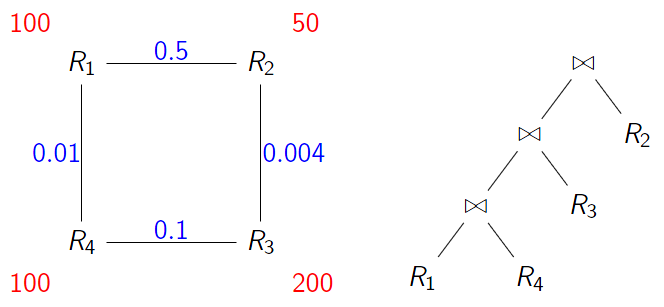
\includegraphics[scale=.6]{graph-and-tree}\\
We assume left deep trees with a commutativity rule set containing $swap$ and $3cycle$.
The costs for all possible join trees can be found in \verb|costs.txt| (as swapping the relations of the first join doesn't change $C_{out}$, these permutations are left out).
A start solution that is a local minimum and therefore wouldn't yield an optimal solution is e.g. $(1 \Join 4)\Join 3)\Join 2$. With $swap$ we can reach $(3 \Join 4)\Join 1)\Join 2$ and $(1 \Join 2)\Join 3)\Join 4$ and with $3cycle$ $(3 \Join 4)\Join 2)\Join 1$ and $(4 \Join 3)\Join 1)\Join 2$ which all have higher costs. Thus the optimal solution $(2 \Join 3)\Join 4)\Join 1$ can't be reached.


\lstinputlisting[caption={Costs for all possible join trees},label=lst:costs]{costs.txt}


\end{document}
